\documentclass[11pt]{article}
\usepackage{amssymb}
\usepackage{amsfonts}
\usepackage{amsmath}
\usepackage{bm}
\usepackage{latexsym}
\usepackage{epsfig}
\usepackage{tikz}

\setlength{\evensidemargin}{.25in}
\setlength{\textwidth}{6in}
\setlength{\topmargin}{-0.4in}
\setlength{\textheight}{8.5in}


\newcommand{\handout}[5]{
   \renewcommand{\thepage}{#1-\arabic{page}}
   \noindent
   \begin{center}
   \framebox{
      \vbox{
    \hbox to 5.78in {{\sf 18.312: Algebraic Combinatorics} 
\hfill \sf #2 }
       \vspace{4mm}
       \hbox to 5.78in { {\Large \hfill #5  \hfill} }
       \vspace{2mm}
       \hbox to 5.78in { {\em #3 \hfill #4} }
      }
   }
   \end{center}
   \vspace*{4mm}
}

\newcommand{\lecture}[4]{\handout{#1}{#2}{Lecture date: #3}{Notes by: #4}{Lecture #1}}


\textwidth=6in
\oddsidemargin=0.25in
\evensidemargin=0.25in
\topmargin=-0.1in
\footskip=0.8in
\parindent=0.0cm
\parskip=0.3cm
\textheight=8.00in
\setcounter{tocdepth} {3}
\setcounter{secnumdepth} {2}
\sloppy

\newtheorem{theorem}{Theorem}
\newtheorem{lemma}[theorem]{Lemma}
\newtheorem{proposition}[theorem]{Proposition}
\newtheorem{corollary}[theorem]{Corollary}
\newtheorem{fact}[theorem]{Fact}
\newtheorem{definition}[theorem]{Definition}
\newtheorem{remark}[theorem]{Remark}
\newtheorem{conjecture}[theorem]{Conjecture}
\newtheorem{question}[theorem]{Question}
\newenvironment{answer}{\noindent \textbf{Answer:}}{}
\newtheorem{answer2}[theorem]{Answer}
\newtheorem{exercise}[theorem]{Exercise}
\newtheorem{example}[theorem]{Example}
\newenvironment{proof}{\noindent \textbf{Proof:}}{$\Box$}

\newcommand{\N}{\mathbb N} % natural numbers 0,1,2,...
\newcommand{\Z}{\mathbb Z}  % integers
\newcommand{\R}{\mathbb R} % reals
\newcommand{\C}{\mathbb C} % complex numbers
\newcommand{\F}{\mathbb F} % finite fields

\newcommand{\floor}[1]{\left\lfloor {#1} \right\rfloor} % floor function
\newcommand{\ceiling}[1]{\left\lceil {#1} \right\rceil} % ceiling function
\newcommand{\binomial}[2]{\left( \begin{array}{c} {#1} \\ 
                        {#2} \end{array} \right)} % binomial coefficients
\newcommand{\modulo}[1]{\quad (\mbox{mod }{#1})} %congruences

\newcommand{\ignore}[1]{} % useful for commenting things out

%shortcuts added for lecture 20.
\newcommand{\keyword}[1]{{\emph{#1}}}

\begin{document}
\lecture{20}{Lionel Levine}{Apr 26, 2011}{Josh Alman} 

\section{Plan for the Remainder of the Course}

Today: Applications of the Matrix-Tree Theorem
\begin{itemize}
	\vspace{-11pt}
	\item Hamming Cube
	\vspace{-2pt}
	\item Eulerian Tours
	\vspace{-11pt}
\end{itemize}

Next Class: De Bruijn sequences, Polya Theory

\vspace{-2pt}
In-class final on Thurs, May 5$^{th}$

\vspace{-2pt}
Last week: Abelian Sandpile Group

\vspace{-9pt}
\section{Hamming Cube}

Our first application of the Matrix-Tree Thorem will be to find the number of spanning trees in the Hamming Cube.

\begin{definition}
	The \keyword{Hamming Cube of dimension $n$}  is the undirected graph $H_n = (V,E)$, where
	$V=\{0,1\}^n$ is the set of binary strings of length $n$, and $x,y \in V$ are adjacent iff
	$x_i = y_i$ for all but one index $i \in [n]$.
\end{definition}

\begin{example}
	For $n=3$, we have that $H_3$ looks like:
	

	\begin{figure}[ht]
    \begin{center}
    \begin{tikzpicture}
        \tikzstyle{every node} = [rectangle]
        \node (000) at (-1,-1) {$000$};
        \node (001) at (-1,1) {$001$};
        \node (010) at (1,-1) {$010$};
        \node (011) at (1,1) {$011$};
        \node (100) at (0,0) {$100$};
        \node (101) at (0,1.9) {$101$};
        \node (110) at (1.9,0) {$110$};
        \node (111) at (1.9,1.9) {$111$};
        
        \foreach \from/\to in {000/001, 000/010, 000/100, 001/011, 001/101,
        010/011, 010/110, 100/101, 100/110, 011/111, 101/111, 110/111}
            \draw[-] (\from) -- (\to);
    \end{tikzpicture}
    \end{center}
    \caption{The Hamming Cube of dimension 3.}
	\end{figure}

\end{example}

\begin{question}
	How many spanning trees are there in $H_n$?
\end{question}

\begin{answer}
	By the Matrix-Tree Theorem, the number of spanning trees is given by:
	\begin{equation} \label{eval} \kappa(H_n) = \frac{\lambda_1 \cdot \lambda_2 \dotsb \lambda_{N-1}}{N}, \end{equation}
	where $N=|V|=2^n$ is the number of vertices, and $\lambda_1, ... \lambda_{N-1}$
	are the non-zero eigenvalues of the Laplacian matrix:
	$$L=nI-A_n,$$
	where $A_n$ is the adjacency matrix for $H_n$. Indeed, each vertex has degree $n$
	since it is adjacent to the vertex which differs from it only in the $i^{th}$ position
	for all $i \in [n]$. 
	
	Now, we are going to find the eigenvalues of $A_n$ by finding the eigenvalues of $A_1$ and
	writing the eigenvalues of $A_n$ as sums of these. Notice that:
	$$H_n = H_1 \times H_1 \times \dotsb \times H_1 \qquad (n \text{ times}).$$
	This gives us exactly that two vertices in $H_n$ are adjacent if they differ in exactly
	one position, as we want. Thus, we get that:
	\begin{equation} \label{tense} A_n = A_1 \otimes I \otimes I \otimes \dotsb \otimes I + I \otimes A_1 \otimes I \otimes \dotsb \otimes I + \dotsm + I \otimes I \otimes I \otimes \dotsb \otimes I \otimes A_n. \end{equation}
	One might think that we actually get $A_n = A_1 \otimes A_1 \otimes \dotsb \otimes A_1 \quad (n \text{ times})$, but
	this would actually correspond to the graph where two binary strings are adjacent if they
	differ in every position. We can see that (\ref{tense}) is correct.
	
	Now, $H_1$ looks like:
	
	\begin{figure}[ht]
    \begin{center}
    	\begin{tikzpicture}
        \tikzstyle{every node} = [rectangle]
        \node (0) at (-1,0) {$0$};
        \node (1) at (1,0) {$1$};
        
        \foreach \from/\to in {0/1}
            \draw[-] (\from) -- (\to);
    	\end{tikzpicture}
    \end{center}
    \caption{The Hamming Cube of dimension 1.}
	\end{figure}
	
	This has adjacency matrix:
	$$A_1= \begin{pmatrix} 0 & 1 \\ 1 & 0 \end{pmatrix}.$$
	Letting $v_1 = \begin{pmatrix} 1 \\ 1 \end{pmatrix}$ and $v_2 = \begin{pmatrix} 1 \\ -1 \end{pmatrix}$, we can see that:
	$$A_1v_1 = v_1, \text{ and } A_1v_2=-v_2,$$
	so $A_1$ has eigenvectors $v_1$ and $v_2$ with eigenvalues $1$ and $-1$, respectively. Thus, by
	(\ref{tense}), we get that the eigenvectors of $A_n$ are the vectors of the form:
	$$v = v_{i_1} \otimes v_{i_2} \otimes \dotsb \otimes v_{i_n}, \qquad \text{ where } i_r \in \{1,2\} \text{ } \forall r \in [n].$$
	The corresponding eigenvalue for this eigenvector of $A_n$ is simply the sum of the eigenvalues of the  '$v_{i_r}$'s,
	which is:
	$$\lambda_v = \sum_{i_r = 1}1 + \sum_{i_r = 2}(-1)$$
	$$=n-2\cdot \#\{r \text{ }| \text{ } i_r = 2\}.$$
	Thus, since there are $\binom{n}{k}$ ways to pick $k$ of the $n$ '$i_r$'s to equal $2$,
	we have that $A_n$ has the eigenvalue $n-2k$ with multiplicity $\binom{n}{k}$ for each $k=0,1,...,n$;
	this is all the $2^n$ eigenvalues of $A_n$. Recalling that:
	$$L_n=nI-A_n,$$
	we get that $L_n$ has eigenvalue $n-(n-2k)=2k$ with multiplicity $\binom{n}{m}$ for each $k=0,1,...,n$.
	We can finally evaluate (\ref{eval}), keeping in mind that we do not include zero eigenvalues in our product:
	\begin{equation} \label{ans} \kappa(H_n) = \frac{\prod_{k=1}^n (2k)^{\binom{n}{k}}}{N} = \frac{\prod_{k=1}^n (2k)^{\binom{n}{k}}}{2^{\binom{n}{1}}} = \prod_{k=2}^n (2k)^{\binom{n}{k}} \end{equation}
	Thus, the number of spanning trees in $H_n$ is \framebox[1in]{$\prod_{k=2}^n (2k)^{\binom{n}{k}}$.}
\end{answer}

Surprisingly, despite the form of this answer, finding a combinatorial proof of it is an open problem. One
promising approach involves corresponding spanning trees in $H_n$ to phototropic trees in $H_n$ - trees where
the sun is placed at the origin, and edges "grow toward the light." More formally:

\begin{definition}
	A directed spanning tree $T_n$ of $H_n$, rooted at the origin, $0^n$, is called
	\keyword{phototropic} if whenever the arc $(x,y) \in T_n$, we have that $x_i \geq y_i \text{ } \forall i \in [n]$.
\end{definition}

\begin{example}
	Here are directed spanning trees in $H_2$:

	\begin{figure}[ht]
    \begin{center}
    	\begin{tikzpicture}
        \tikzstyle{every node} = [rectangle]
        \node (00) at (1,1) {$00$};
        \node (01) at (-1,1) {$01$};
        \node (10) at (1,-1) {$10$};
        \node (11) at (-1,-1) {$11$};
        \foreach \from/\to in {01/00, 10/00, 11/01}
            \draw[->] (\from) -- (\to);
    	\end{tikzpicture}
    \end{center}
    \caption{A phototropic tree in $H_2$}
	\end{figure}


\pagebreak


	\begin{figure}[ht]
  	\begin{center}   
    	\begin{tikzpicture}
        \tikzstyle{every node} = [rectangle]
        \node (00) at (1,1) {$00$};
        \node (01) at (-1,1) {$01$};
        \node (10) at (1,-1) {$10$};
        \node (11) at (-1,-1) {$11$};
        \foreach \from/\to in {01/00, 10/11, 11/01}
            \draw[->] (\from) -- (\to);
    	\end{tikzpicture}
    
    \end{center}
    \caption{A tree in $H_2$ that is not phototropic, since there is an arc between $10$ and $11$ in the wrong direction.}
	\end{figure}
	
\end{example}

Counting phototrpphic trees is simple: we can construct them by choosing an outward arc for each vertex other than the origin. The arc from a vertex $x$ must go to a vertex identical to $x$ except that it has a zero in one position where $x$ has a one, and so if there are $a_x$ ones in $x$, then there are $a_x$ choices for that arc. The number of phototropic trees in $H_n$ is thus:

$$ \#\{\text{phototropic trees in }H_n\} = \prod_{x \in \{0,1\}^n \backslash 0^n} a_x = \prod_{x \in \{0,1\}^n \backslash 0^n} \left(\sum_{i=1}^n x_n \right) = \prod_{k=1}^n k^{\binom{n}{k}} $$

The similarity of this answer to (\ref{ans}) leads to the idea of corresponding phototropic trees to spanning trees to produce a combinatorial proof of our earlier result.


\section{Eulerian Tours}
\subsection{Introducing the problem}

In this section, we will use a tricky application spanning trees to find the number of Eulerian tours in a directed graph.

\begin{definition}
	If $G = (V,E)$ is a finite directed graph, with $n=|V|, m=|E|$, then a \keyword{(directed) Eulerian tour} of G is a path $t_0, t_1, ..., t_m=t_0$ with each $t_i \in V$, such that each directed edge is used exactly once, meaning, 																$\{(t_i,t_{i+1})\}_{i=0}^{m-1}=E$.
\end{definition}

\begin{example}
	Here are some Eulerian tours on $\overleftrightarrow{K_3}$: 
	

	\begin{figure}[ht]
    \begin{center}
    	\begin{tikzpicture}
        \tikzstyle{every node} = [rectangle]
        \node (0) at (-1,-1) {$0$};
        \node (1) at (1,-1) {$1$};
        \node (2) at (0,.7) {$2$};        
        \draw[->] (-0.7,-1) -- (0.7,-1);
        \draw[->] (0.7,-0.8) -- (-0.7,-0.8);
        \draw[->] (1,-0.8) -- (0.2, 0.7);
        \draw[->] (0.1, 0.6) -- (0.9,-0.9);
        \draw[->] (-0.2, 0.7) -- (-1,-0.8);
        \draw[->] (-0.9,-0.9) -- (-0.1, 0.6);
    	\end{tikzpicture}
    \end{center}
    \caption{The complete directed graph on 3 vertices.}
	\end{figure}
	
	
	\begin{figure}[ht]
    \begin{center}
    	\begin{tikzpicture}
        \tikzstyle{every node} = [rectangle]
        \node (0) at (-1.2,-1.2) {$0$};
        \node (1) at (1.2,-1.2) {$1$};
        \node (2) at (0,1.1) {$2$};        
        
				\draw[->] (-1,-1) -- ++(1,1.7) -- ++(1,-1.7) -- ++(-1.8,0) -- ++(0,0.2) -- ++(1.5,0) -- ++(-0.7,1.19) -- ++(-0.6,-1.02);
    	\end{tikzpicture}
    \end{center}
    \caption{The Eulerian Tour 021012}
	%\end{figure}
	
	
	
	%\begin{figure}[ht]
    \begin{center}
    	\begin{tikzpicture}
        \tikzstyle{every node} = [rectangle]
        \node (0) at (-1.2,-1.2) {$0$};
        \node (1) at (1.4,-1.2) {$1$};
        \node (2) at (0.1,1.1) {$2$};        
        
				\draw[->] (-1,-1) -- ++(1,1.7) -- ++(0,-0.3) -- ++(-0.7,-1.19) -- ++(1.6,0) -- ++(-0.7,1.19)
									-- ++(0,0.3) -- ++(1,-1.7) -- ++(-2.0,0);
    	\end{tikzpicture}
    \end{center}
    \caption{The Eulerian Tour 020121}
	\end{figure}

\end{example}


\pagebreak

\begin{question}
	Which directed graphs have Eulerian tours?
\end{question}

One might recall that an undirected graph has an Eulerian tour if every vertex has even degree. However, here, we are dealing with directed graphs, so the condition will require that our graph be balanced.

\begin{definition}
	In a directed graph $G=(V,E)$, a vertex $v \in V$ is said to be \keyword{balanced} if it has equal indegree and outdegree;
	$$\text{indeg}(v)=\text{outdeg}(v).$$
\end{definition}

\begin{definition}
	A directed graph $G=(V,E)$ is said to be \keyword{balanced} if each of its vertices is balanced.
\end{definition}

We can then state our condition on a directed graph having an Eulerian tour:

\begin{answer2}
	A directed graph G=(V,E) has an Eulerian tour iff it is balanced.
\end{answer2}

It is clear that a directed graph needs to be balanced to have an Eulerian tour. The converse ends up being true as well. We will see this, but we also want to count the number of Eulerian tours in a directed graph that has any.

\begin{definition}
	If $G=(V,E)$ is a directed graph, with $e \in E$ an arc in the graph, then we write:
	$$\tau(G,e):=\#\{\text{Eulerian tours of }G \text{ starting with the edge } e\}.$$
\end{definition}

Since an Eulerian tour goes over all arcs in a graph, and we can cycle our tours to start at any edge we want, we can see that $\tau(G,e)$ is actually independent of $e$, so we can similarly define $\tau(G) := \tau(G,e)$ for any $e \in E$. Recalling that $\kappa(G,v_0)$ is the number of oriented spanning trees in directed graph $G$ rooted at vertex $v_0$, we can then state our theorem for counting Eulerian tours in directed graphs:

\begin{theorem}
	If $G=(V,E)$ is a directed graph, then $G$ has an Eulerian tour iff it is balanced. If it is balanced, then for any $e=(v_0,v_1)\in E,$
	\begin{equation} \label{theo} \tau(G) = \tau(G,e) = \kappa(G,v_0)\cdot \prod_{v \in V} (deg(v) - 1)!.\end{equation}
\end{theorem}

We quickly introduce some new notation:

\begin{definition}
	If $e \in E$ is an arc in directed graph $G=(V,E)$, and $e=(v,w)$, then we write:
	$$e^-:=v,$$
	$$e^+:=w.$$
	Then, for a vertex $x \in V$, we write $E_x$ for the set of arcs coming out of $x$:
	$$E_x := \{ f \in E | f^-=x \}.$$
\end{definition}

We want to interpret the $(deg(v) - 1)!$ terms in (\ref{theo}) as cyclic permutations of the edges in $E_v$. We thus define the following:

\begin{definition}
	Given an Eulerian tour $\gamma=(t_0,t_1,...,t_{m-1})$ in directed graph $G=(V,E)$, for any vertex $v \in V$, let $i_1,...,i_d$ be 	the indices such that $t_{i_r}=v, r=1,...,d = outdeg(v)$. Then, for each $r$, write $e_r = (v,t_{i_r+1})$; the '$e_r$' are the 	edges in $E_v$ in the order that they are crossed in $\gamma$. Then, we can define the cyclic permutation $c_v: E_v \rightarrow 		E_v$ as:
	$$c_v(e_r) = \begin{cases}
														e_{r+1} & \text{if } 1 \leq r < d \\
														e_1			&	\text{if } r = d
							 \end{cases}$$
\end{definition}

To use this new cyclic permutation, we are going to use some properties of Rotor Walks.

\subsection{Rotor Walks}

\begin{definition}
	A \keyword{rotor configuration} on a directed graph $G=(V,E)$ is a map $\rho:V \rightarrow E$ such that $\rho(v) \in E_v \text{  } 	\forall v \in v$; it assigns an outgoing edge to each vertex.
\end{definition}

\begin{definition}
	Given a directed graph $G=(V,E)$ and associated $\rho$ and a $c_v$ for each $v \in V$, and a starting vertex $V_0$, define a \keyword{rotor walk} as a sequence of vertices in $V$, $v_0, v_1, v_2, ...$, as follows: let $\rho_0 = \rho$, then for each $i=1,2,...,$ let:
	$$\rho_i(w)= \begin{cases}
														\rho_{i-1}(w) 										& \text{if } w \neq v_{i-1} \\
														c_{v_{i-1}}(\rho_{i-1}(v_{i-1}))	&	\text{if } w=v_{i-1}.
							 \end{cases}$$
	Then, let $v_i = \rho_i(v_{i-1})^+$.
\end{definition}

Basically, at each step, the rotor of the vertex we are looking at goes to the next edge coming out of that vertex in its cyclic permutation of edegs, and we move along that new edge. We illustrate this with an example on $\overleftrightarrow{K_3}$:

\pagebreak

\begin{example}

We give the initial conditions in $\rho_0$; at each step, the arcs in the current $\rho$ are shown:
	
	\begin{figure}[h!]
    \begin{center}
    	\begin{tikzpicture}
        \tikzstyle{every node} = [rectangle]
        \node (0) at (-1,-1) {$-$};
        \node (1) at (1,-1) {$-$};
        \node (2) at (0,.7) {$v_0$}; 
               
        \foreach \from/\to in {0/2, 2/0, 1/0}
            \draw[->] (\from) -- (\to);
      \end{tikzpicture}
    \end{center}
    \caption{$\rho_0$}
    
    
    \begin{center}
    	\begin{tikzpicture}
        \tikzstyle{every node} = [rectangle]
        \node (0) at (-1,-1) {$-$};
        \node (1) at (1,-1) {$v_1$};
        \node (2) at (0,.7) {$v_0$}; 
               
        \foreach \from/\to in {0/2, 2/1, 1/0}
            \draw[->] (\from) -- (\to);
      \end{tikzpicture}
    \end{center}
    \caption{$\rho_1$}

    
    \begin{center}
    	\begin{tikzpicture}
        \tikzstyle{every node} = [rectangle]
        \node (0) at (-1,-1) {$-$};
        \node (1) at (1,-1) {$v_1$};
        \node (2) at (0,.7) {$v_0=v_2$}; 
               
        \foreach \from/\to in {0/2, 2/1, 1/2}
            \draw[->] (\from) -- (\to);
      \end{tikzpicture}
    \end{center}
    \caption{$\rho_2$}

    
    \begin{center}
    	\begin{tikzpicture}
        \tikzstyle{every node} = [rectangle]
        \node (0) at (-1,-1) {$v_3$};
        \node (1) at (1,-1) {$v_1$};
        \node (2) at (0,.7) {$v_0=v_2$}; 
               
        \foreach \from/\to in {0/2, 2/0, 1/2}
            \draw[->] (\from) -- (\to);
      \end{tikzpicture}
    \end{center}
    \caption{$\rho_3$}

	\end{figure}
	\begin{figure}[h!]
    
    \begin{center}
    	\begin{tikzpicture}
        \tikzstyle{every node} = [rectangle]
        \node (0) at (-1,-1) {$v_3$};
        \node (1) at (1,-1) {$v_1=v_4$};
        \node (2) at (0,.7) {$v_0=v_2$}; 
               
        \foreach \from/\to in {0/1, 2/0, 1/2}
            \draw[->] (\from) -- (\to);
      \end{tikzpicture}
    \end{center}
    \caption{$\rho_4$}

    
    \begin{center}
    	\begin{tikzpicture}
        \tikzstyle{every node} = [rectangle]
        \node (0) at (-1,-1) {$v_3=v_5$};
        \node (1) at (1,-1) {$v_1=v_4$};
        \node (2) at (0,.7) {$v_0=v_2$}; 
               
        \foreach \from/\to in {0/1, 2/0, 1/0}
            \draw[->] (\from) -- (\to);
      \end{tikzpicture}
    \end{center}
    \caption{$\rho_5$}

    
    \begin{center}
    	\begin{tikzpicture}
        \tikzstyle{every node} = [rectangle]
        \node (0) at (-1,-1) {$v_3=v_5$};
        \node (1) at (1,-1) {$v_1=v_4$};
        \node (2) at (0,.7) {$v_0=v_2=v_6$}; 
               
        \foreach \from/\to in {0/2, 2/0, 1/0}
            \draw[->] (\from) -- (\to);
      \end{tikzpicture}
    \end{center}
    \caption{$\rho_6$}

	\end{figure}
	
\end{example}

\pagebreak


Since $\rho_0 = \rho_6$ and $v_0 = v_6$, we are now going to repeat; rotor walking is deterministic. Notice that the vertices traversed on the path, $(v_0, v_1, v_2, v_3, v_4, v_5)$ = $(2,1,2,0,2,1)$, form an Eulerian path of the graph! It turns out that 
the reason for this is that $\rho_0$ formed a spanning tree of the graph.

\subsection{Finding the number of directed Eulerian tours}

\begin{lemma}
	If directed graph $G=(V,E)$ is balanced, and the graph $T=(V, \rho(V-\{v_0\}))$ is a tree, then there exists an Eulerian tour $t_0, t_1, ..., t_{m-1}$ such that the rotor walk $v_0, v_1, v_2, ...$ induced by $\rho$ travels around the tour, namely:
	\begin{align*} v_0=t_0,&\ldots,v_{m-1}=t_{m-1} \\ v_m=t_0, &\ldots, v_{2m-1}=t_{m-1} \\ &\ldots \\  v_{i} = t_{i+m} &\qquad \forall i \geq 0. \end{align*}
\end{lemma}

\begin{proof}
	Let $e=(v_i,v_{i+1})$ be the first edge travelled twice by the rotor walk; $i$ is the smallest index such that $\exists j<i$ such 	that $v_j=v_i$ and $v_{j+1}=v_{i+1}.$ This is well-defined since there are finitely many edges and the path is infinite. Let 				$d=deg(v_i)$. Since each outgoing edge of $v_i$ had to be traversed before $e$ could be traversed a second time, as the rotor goes 	 over all these edges, after step $i$, there have been $d+1$ exits from $v_i$. This means there were $d+1$ entrances to $v_i$. But, 	since $v$ is balanced, there are only $d$ edges coming into it, so one of these edges were already traversed twice, a 							contradiction, unless $v_i=v_0$, as we start there. Thus, the first edge travelled twice started from $v_0$.
	
	Now, we call a vertex $w$ full if all its incoming edges have been used before time $i$, meaning, for each edge $e$ such that 			$e^+=w,$ there exists a $j<i$ such that $e=(v_j,v_{j+1})$. Note that $v_0$ is full, since it had $d$ entrances other than at the 	 	 beginning, and $d$ incoming edges, and none of these were traversed twice.
	
	Notice that if a vertex $w$ is full, and $(u,w)$ is an edge of our initial spanning tree $T$, then $u$ is also full if it is not 		$v_0$. Indeed, $(u,w) \in T$ means that $\rho_0(u)=(u,w)$, meaning $(u,v)$ is the last edge traveled out of $u$ in the rotor walk. 	 But, since $w$ is full, $(u,w)$ was used, so all the edges out of $u$ were used. Thus, there were $deg(u)$ entrances to $u$, and 		since $u$ is not $v_0$, all incoming edges were used, so $u$ is full.
	
	We have that the root of the spanning tree is full, and every non-root vertex adjacent to a full vertex in the tree is full. Since 	 $T$ is a spanning tree, all the vertices are full. Thus, each edge was used exactly once.
\end{proof}

We can now prove our theorem! We recall what we wanted to show:

\begin{theorem}
	If $G=(V,E)$ is a directed graph, then $G$ has an Eulerian tour iff it is balanced. If it is balanced, then for any $e=(v_0,v_1)\in E,$
	\begin{equation} \label{theo2} \tau(G) = \tau(G,e) = \kappa(G,v_0)\cdot \prod_{v \in V} (deg(v) - 1)!.\end{equation}
\end{theorem}

\begin{proof}
We define a bijection:
$$f: \{\text{Eulerian tours of } G \text{ starting with edge } e=(v_0,v_1) \} \rightarrow \qquad $$
$$\qquad \qquad \qquad		\rightarrow \{\text{oriented spanning trees of } G \text{ rooted at } v_0 \} \times \prod_{v \in V} \{\text{cyclic permutations of } E_v \},$$
where the products in the right hand side are cartesian products of sets. Proving this will clearly imply (\ref{theo2}).

We can define $f^{-1}$ as: $f^{-1}(\rho,(c_v)_{v \in V}) \rightarrow \text{rotor walk } (v_0,v_1,...)$, where the rotor walk is exactly what we defined in the lemma. Notiice that an oriented spanning tree does not actually give us a value for $\rho(v_0)$, but we can define it as $\rho(v_0)=c_{v_0}^{-1}(v_0,v_1)$. 

We can define $f$ as: $f(t_0,t_1,...,t_{m-1}) = (\rho, (c_v)_{v \in V})$, where the '$c_v$' are the orders of the edges taken in the tour, and $\rho(u)$ is the last edge travelled out of $u$ in the tour; $\rho(u) = (u,w)$, where $w=v_{M+1}$, where $M=max\{i<m|v_i=u\}$. With $\rho$ defined in this way, $(V,\rho(V-\{v_0\}))$ is a tree because given $S\subset V-\{v\}$, letting $N=max\{i<m|v_i \in S\}$, we have that $(v_N,v_{N+1})$ is an edge of $T$ and $v_{N+1} \notin S$. Thus, $S$ does not form an oriented cycle, and so $T$ is a tree.

It is clear that these are inverses.
\end{proof}

It is worth noting that it is not clear that the number of oriented spanning trees rooted at $v$ is independent of $v$; this is problem PF6 on the practice final.

\end{document}



